\item Water in a canal, $6$ m wide and $1.5$ m deep,is flowing with a speed of $10 \,\text{km/hr}$. How much area will it irrigate in $30$ minutes; if $8$ cm standing water is needed?
\item A man in a boat rowing away from a light house $100m$  high takes $2$ minutes to change the angle of elevation of the top of the light house from $60\degree$ to $30\degree$. Find the speed of the boat in metres per minute. [Use $\sqrt{3}=1.732$]
\item Two poles of equal heights are standing opposite each other on either side of the road, which is $80 m$  wide. From a point between them on the road, the angles of elevation of the top of the poles are $60\degree$ to $30\degree$ respectively. Find the height of the poles and the distances of the point from the poles.
\item A bucket open at the top is in the form of a frustum of a cone with a capacity of $12308.8 cm^3$. The radii of the top and bottom of circular ends of the bucket are $20 cm$ and $12cm$ respectively. Find the height of the bucket and also the area of the metal sheet used in making it. (Use  $\pi= 3.14$)
\item Find the area of the shaded region in \figref{fig:figure445}, if $ABCD$ is a rectangle with sides $8 cm$ and $6 cm$ and $\vec{O}$ is the centre of circle. ($\pi = 3.14$)
\begin{figure}[H]                                     \centering
	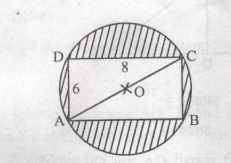
\includegraphics[width=\columnwidth]{figs/i1.jpeg}
		\caption{}
		\label{fig:figure445}

                \end{figure}
\item If $P$ and $Q$ are the points on side $CA$ and $CB$ respectively of  $ABC$, right angled at $C$, prove that $\brak{AQ^2 + BP^2} = \brak{AB^2 +PQ^2}$
\end{enumerate}
